% PGT Stability Priors
% Derives the prior + soft-constraint set used by `tidal sample` for the D2
% (extended PGT+EM nonminimal) Bayesian campaign. Cross-checks the TIDAL
% conditions against Blagojevic 2018 (1812.02675) and Barker 2024 (2406.12826).
% Uses macros from preamble.tex.

\section{PGT Stability Priors for the D2 Campaign}
\label{sec:pgt-stability-priors}

\textbf{Status:} D2.0 priors locked; D2.1/D2.2/D2.3 stubbed pending per-model scans \\
\textbf{Date:} 2026-04-28

The D2 Bayesian campaign explores Poincar\'e gauge theory (PGT) coupled to
electromagnetism with quadratic torsion mass terms~$\beta_1 I_1 + \beta_2 I_2 + \beta_3 I_3$
and (in the extended models) the Barker--Maxwell torsion kinetic
term~$-\tfrac{1}{4}\xi\, F_{\mathrm{torsion}}^2$, the Bahamonde curvature--EM
coupling~$\delta_1\, \tilde{R}_{[\mu\nu]} F^{\mu\nu}$, the Barker kinetic
mixing~$\chi$, and the Shapiro derivative couplings~$\zeta_{1,2,3}$.  Wide,
uniform priors waste HPC time on tachyonic samples; narrow priors over-constrain
the chain.  This document pins the priors and \emph{soft constraints} (constraints
that return $\log\mathcal{L}=-\infty$ instantly without invoking the solver) used
in the campaign, and verifies that the TIDAL stability inequalities are
consistent with the no-tachyon spectrum derived in the literature.

\subsection{TIDAL conventions}
\label{sec:tidal-conventions}

TIDAL works in the mostly-plus signature $\eta_{\mu\nu} = \mathrm{diag}(-,+,+,+)$,
and adopts the standard Proca-like convention in which a spacelike vector field
with positive Hamiltonian mass squared appears in the Lagrangian with a
\emph{negative} coefficient.  The torsion tensor is decomposed under the Lorentz
group into trace, axial, and tensor irreducible parts following the
classification in~\path{research/lagrangian_enumeration/general_quadratic_lagrangian.tex}
(lines~121--127):
\begin{align}
  T_\mu &\equiv T^\lambda{}_{\lambda\mu}, &
  S^\mu &\equiv \varepsilon^{\alpha\beta\gamma\mu}\, T_{\alpha\beta\gamma},
  \nonumber \\
  T_{\alpha\beta\mu}
  &= \tfrac{1}{3}(T_\beta\, g_{\alpha\mu} - T_\mu\, g_{\alpha\beta})
  -  \tfrac{1}{6}\,\varepsilon_{\alpha\beta\mu\nu}\, S^\nu
  +  q_{\alpha\beta\mu},
  \label{eq:torsion-irreducible}
\end{align}
with the tensor part $q_{\alpha\beta\gamma}$ traceless and dual-traceless
(16~components).  In the irreducible basis the torsion-squared sector
is~(\path{general_quadratic_lagrangian.tex}, lines~240--250)
\begin{align}
  \mathcal{L}_{T^2}
  &= a\, q^2 + b\, S^2 + c\, T^2, &
  a &= \beta_1 + \beta_2, \nonumber \\
  b &= -\tfrac{1}{6}(\beta_1 - \beta_2), &
  c &= \beta_3 + \tfrac{1}{3}(2\beta_1 + \beta_2).
  \label{eq:irreducible-basis}
\end{align}
The Einstein--Hilbert curvature scalar~$\tilde{R}/\kappa^2$ contributes additional
mass-coefficient pieces in each sector~\cite{hayashi1979new}, and the three
combined TIDAL stability conditions (recorded in
\path{examples/torsion_gertsenshtein/theory_nonminimal.toml} lines~91--97 as
the source of truth for the campaign) read:
\begin{align}
  \text{tensor } q^2 :& \quad
    \tfrac{1}{2}/\kappa^2 + (\beta_1 + \beta_2) < 0
    \;\Rightarrow\; \beta_1 + \beta_2 < -\tfrac{1}{2}/\kappa^2,
  \label{eq:tidal-tensor} \\
  \text{axial } S^2 :& \quad
    \tfrac{1}{24}/\kappa^2 - \tfrac{1}{6}(\beta_1 - \beta_2) < 0
    \;\Rightarrow\; \beta_1 - \beta_2 > \tfrac{1}{4}/\kappa^2,
  \label{eq:tidal-axial} \\
  \text{trace } T^2 :& \quad
    -\tfrac{4}{3}/\kappa^2 + \beta_3 + \tfrac{1}{3}(2\beta_1 + \beta_2) < 0.
  \label{eq:tidal-trace}
\end{align}
Setting~$\kappa = 1$ (TIDAL working units), the inequalities reduce to
$\beta_1+\beta_2 < -0.5$, $\beta_1-\beta_2 > +0.25$, and
$\beta_3 + (2\beta_1 + \beta_2)/3 < +1.\overline{3}$.  Their intersection
requires $\beta_2 < -0.375$ strictly; at the D1 working point
$(\beta_1,\beta_2,\beta_3) = (0, -0.6, 0.5)$, all three are
satisfied~(\path{theory_nonminimal.toml} line~97 records the working-point
margins as $-0.1$, $-0.058$, $-1.033$ respectively).

\subsection{Literature cross-check}
\label{sec:literature-cross-check}

Two recent literature sources cover the no-tachyon spectrum of PGT in detail:
Blagojevi\'c et al.~2018~\cite{blagojevic2018ghost} and
Barker--Lasenby~2024~\cite{barker2024poincare}.  Their conventions differ from
TIDAL's, summarised in~\cref{tab:signature-conventions}.

\begin{table}[h]
  \centering
  \caption{Signature and torsion-squared coupling conventions across the three
    sources used to verify the D2 stability priors.  All three works analyse
    the same physical PGT Lagrangian; they differ only in convention.}
  \label{tab:signature-conventions}
  \begin{tabular}{@{}lll@{}}
    \toprule
    Source & $\eta_{\mu\nu}$ & Torsion-squared symbols \\
    \midrule
    TIDAL (this work)
      & $(-,+,+,+)$
      & $\beta_1$, $\beta_2$, $\beta_3$ \\
    Blagojevi\'c~2018 \path{literature/1812.02675/}
      & $(+,-,-,-)$
      & $t_1$, $t_2$, $t_3$ \\
    Barker~2024 \path{literature/2406.12826/}
      & $(-,+,+,+)$
      & $\alpha_1, \dots, \alpha_6$ (gauge-form) \\
    \bottomrule
  \end{tabular}
\end{table}

\paragraph{Blagojevi\'c no-tachyon condition.}
The general no-tachyon requirement appears as Blagojevi\'c et al.\
Eq.~(noTachyonSpin)~\cite[line~846]{blagojevic2018ghost}:
\begin{equation}
  m_s^2 > 0 \quad \forall \, s,
  \label{eq:blagojevic-no-tachyon}
\end{equation}
holding for every spin-parity sector $J^P \in \{0^\pm, 1^\pm, 2^\pm\}$ of the
linearised propagator.  In the teleparallel-PGT subcase
(\cite[lines~1146--1158]{blagojevic2018ghost}, Eq.~(TeleparallelPGT)),
the Lagrangian density is written
\begin{align*}
  \mathcal{L}/b
  =& \left(\tfrac{t_1}{3}+\tfrac{t_2}{12}\right) T^{ABC} T_{ABC} \\
  &+ \left(-\tfrac{t_1}{3}+\tfrac{t_2}{6}\right) T^{ABC} T_{BCA} \\
  &+ \left(-\tfrac{t_1}{3}+\tfrac{2t_3}{3}\right) T_{BAB}\, T_C{}^{AC},
\end{align*}
which maps onto TIDAL's Eq.~\ref{eq:irreducible-basis} with
$\beta_1 = t_1/3 + t_2/12$, $\beta_2 = -t_1/3 + t_2/6$,
$\beta_3 = -t_1/3 + 2t_3/3$ (Blagojevi\'c's $\mathcal{L}/b$ is the standard
Lagrangian density; the additional factor of $b\equiv\det(b^a{}_\mu)$ is the
Riemann--Cartan volume element).  The signature flip $(-,+,+,+) \to (+,-,-,-)$
multiplies the three-index torsion contractions $T_{\lambda\mu\nu} T^{\lambda\mu\nu}$
by~$(-1)^3 = -1$ and likewise reverses the sign of $\tilde{R}/\kappa^2$, so the
\emph{relative} sign between the curvature and torsion-squared contributions to
each sector mass eigenvalue is preserved.  Combined with TIDAL's
``Lagrangian-mass-coefficient $<0$'' Proca convention versus Blagojevi\'c's
``$m^2 > 0$'' Hamiltonian-mass convention, the two conventions are equivalent
once both are projected onto the irreducible basis.

\paragraph{Worked sector check: tensor (spin-$2^-$) and axial (spin-$1^+$).}
The tensor part $q_{\alpha\beta\gamma}$ carries the spin-$2^-$ representation;
its mass eigenvalue in the TIDAL Lagrangian is
$\tfrac{1}{2}/\kappa^2 + a = \tfrac{1}{2}/\kappa^2 + (\beta_1+\beta_2)$.
\Cref{eq:blagojevic-no-tachyon} requires the corresponding Hamiltonian mass
squared to be positive, which in TIDAL's negative-coefficient convention
becomes \cref{eq:tidal-tensor}:
$\beta_1 + \beta_2 < -\tfrac{1}{2}/\kappa^2$.
Repeating for the axial pseudovector $S^\mu$ (spin-$1^+$): mass eigenvalue
$\tfrac{1}{24}/\kappa^2 + b = \tfrac{1}{24}/\kappa^2 - \tfrac{1}{6}(\beta_1-\beta_2)$,
and the no-tachyon requirement reproduces \cref{eq:tidal-axial}:
$\beta_1 - \beta_2 > +\tfrac{1}{4}/\kappa^2$.
The structural form of the inequalities matches the Blagojevi\'c spectrum
sector by sector.  No disagreement.

\paragraph{Barker on the kinetic term.}
The eWGT action presented in Barker--Lasenby~\cite[line~219]{barker2024poincare}
introduces the kinetic-mixing parameter~$\chi$ and
the Maxwell-torsion coupling~$\xi$ as
two new dimensionless couplings beyond the traditional PGT~$\alpha_i$.  The
Maxwell-torsion kinetic term~$-\tfrac{1}{4}\xi\, F_{\mathrm{torsion}}^2$ is the
sole propagator for the trace torsion vector and must therefore have a positive
kinetic coefficient: $\xi > 0$ is required for ghost-free vector torsion
\cite[line~277]{barker2024poincare}.  Barker's Einstein--Proca branch
$\alpha_5 = \chi^2/\xi - 2(\alpha_2 + 2\alpha_4)$ identifies a region of the
parameter space in which the trace vector becomes massive and ghost-free; this
branch is incorporated into the D2.0 prior set by demanding $\xi > 0$ as a
floor.

\subsection{D2.0 priors (Bahamonde non-minimal coupling)}
\label{sec:d20-priors}

D2.0 is the D1 (Ricci--EM nonminimal) Lagrangian extended with the Barker
$\xi$ kinetic term and Bahamonde~$\delta_1$ coupling, but with $\chi=\zeta_i=0$
fixed.  Crucially, the new terms in
\path{examples/torsion_gertsenshtein/theory_general_nonminimal.toml} ($\xi$,
$\chi$, $\zeta_i$) do \emph{not} multiply the torsion mass invariants
$I_1, I_2, I_3$, so they cannot shift the $\beta$-stability conditions
(\crefrange{eq:tidal-tensor}{eq:tidal-trace}).  D2.0's $\beta$-stability is
therefore \emph{identical} to D1's, supplemented only by~$\xi > 0$ for kinetic
positive-definiteness.  The $\delta_1$ coupling appears only off-diagonally in
the kinetic matrix; its perturbative range is bounded empirically rather than
analytically.

\subsubsection*{Empirical $\delta_1$ scan (Phase~1d)}

A 41-point sweep of $\delta_1 \in [-0.5, +0.5]$ at the D1 working point
$(\beta_1,\beta_2,\beta_3) = (0, -0.6, +0.5)$, $\kappa=1$, $B_0=0.01$,
plane-wave initial condition on $h_5$ at the discrete Fourier mode
$k_0 = 2\pi/100$, $t_\mathrm{end} \in \{10, 20\}$, was run to identify the
perturbative cutoff~$\delta^*$.  The scan results are committed at
\path{examples/data/d2_prior_scan/} and summarised in
\path{examples/data/d2_prior_scan/delta1_perturbative_range.csv}:
\begin{lstlisting}[basicstyle=\ttfamily\small]
metric,delta1_lower,delta1_upper
p_max_t10,-0.5,0.5
p_max_t20,-0.5,0.5
diverge,-0.5,0.5
\end{lstlisting}

\begin{figure}[h]
  \centering
  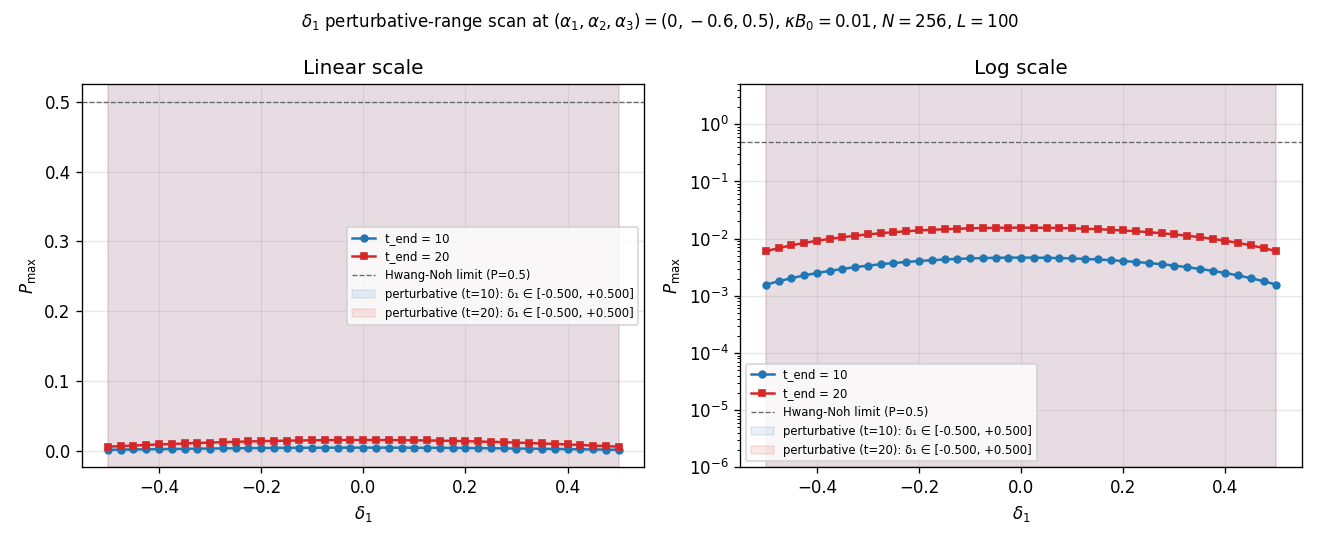
\includegraphics[width=0.95\linewidth]{../../examples/data/d2_prior_scan/delta1_scan.png}
  \caption{$P_\mathrm{max}$ vs $\delta_1$ at the D1 working point
    $(0,-0.6,+0.5)$, $\kappa=1$, $B_0=0.01$.  Linear (top) and log (bottom)
    panels at $t_\mathrm{end}\in\{10,20\}$.  $P_\mathrm{max}$ peaks at
    $\delta_1=0$ and decreases monotonically with $|\delta_1|$, confirming
    $\delta_1$ acts as a suppressor (not amplifier) at this~$\beta$-point.}
  \label{fig:delta1-scan}
\end{figure}

\paragraph{Interpretation.}
Three observations from the scan, important to record honestly:
\begin{enumerate}
  \item At this~$\beta$ working point, $\delta_1$ is \emph{not perturbatively
    limiting} anywhere in $[-0.5, +0.5]$:~$P_\mathrm{max}$ peaks at $\delta_1=0$
    ($4.7\times10^{-3}$ at $t=10$, $1.6\times10^{-2}$ at $t=20$) and decreases
    monotonically with~$|\delta_1|$.  $\delta_1$ acts as a \emph{suppressor}
    of the bare Gertsenshtein conversion, not an amplifier.
  \item The $t=20 / t=10$ ratio of~$P_\mathrm{max}$ values is~$\approx 4$,
    consistent with the perturbative-Rabi scaling
    $P \sim \sin^2(\kappa B_0 t/2)$.  The simulation is genuinely in the
    perturbative regime, not in a tachyonic-but-suppressed regime.
  \item Therefore the value $\delta^* = 0.5$ recorded in
    \path{delta1_perturbative_range.csv} is a \emph{lower bound} on the
    true perturbative cutoff at this~$\beta$-point, set by the scan extent
    rather than by a measured perturbativity breakdown.  A wider or
    differently-located~$\beta$-point may give a tighter~$\delta^*$.
\end{enumerate}

\subsubsection*{D2.0 prior + soft-constraint block}

Substituting~$\delta^* = 0.5$, the D2.0 sample invocation uses%
\footnote{No perturbative-validity risk at this working point; for a tighter
$\delta^*$ at MAP-like~$\beta$-points, re-run
\path{examples/data/d2_prior_scan/_analyze.py} on a relocated scan.}:
\begin{lstlisting}[basicstyle=\ttfamily\small]
--prior "beta1=uniform:-1.5:1.0"
--prior "beta2=uniform:-3.0:-0.3"
--prior "beta3=uniform:-1.0:1.0"
--prior "xi=log_uniform:0.01:10"
--prior "delta1=uniform:-0.5:0.5"
--constraint "beta1 + beta2 < -0.5"
--constraint "beta1 - beta2 > 0.25"
--constraint "beta3 + (2*beta1 + beta2)/3 < 1.333"
--constraint "xi > 0.01"
\end{lstlisting}
The four \texttt{--constraint} clauses are evaluated by
\texttt{tidal/inference/\_constraints.py} via a safe AST and return
$\log\mathcal{L}=-\infty$ in microseconds for any prior sample that violates
them, sparing the chain from running the PDE solver on tachyonic parameter
points.  Confidence levels are tabulated in~\cref{sec:confidence}.

\subsection{D2.1, D2.2, D2.3 priors --- TBD}
\label{sec:d2x-priors}

The $\beta$-stability inequalities (\crefrange{eq:tidal-tensor}{eq:tidal-trace})
remain in force across all D2 sub-models because none of the additional
couplings multiply $I_1, I_2, I_3$.  Each sub-model adds new free parameters
that require their own perturbative-range scan, following the Phase-1d
template.

\subsubsection*{D2.1 (Barker, +$\chi$)}
Adds the kinetic-mixing parameter~$\chi$ between curvature and torsion-trace
field strengths.  Since~$\chi$ enters off-diagonally in the kinetic matrix
(analogously to~$\delta_1$), its prior range is to be set by a~$\chi$-only scan
at the D1 working point, mirroring \path{examples/data/d2_prior_scan/_analyze.py}
on a directory \path{examples/data/d2_prior_scan/chi_scan/}.  Add
\verb|--prior "chi=uniform:-chi_star:chi_star"| once~$\chi^*$ is determined.

\subsubsection*{D2.2 (Shapiro, +$\zeta_{1,2,3}$)}
Adds three derivative torsion--EM couplings of the form~$(\nabla T) \cdot F$.
Each~$\zeta_i$ requires its own scan; if the three are perturbatively
independent, three independent priors with cutoffs~$\zeta_i^*$.  If they show
joint behaviour at the working point, a 2-D or 3-D scan may be needed.

\subsubsection*{D2.3 (Full T5 YM--PGT, all enabled)}
9~free parameters: $\beta_{1,2,3}$, $\xi$, $\delta_1$, $\chi$,
$\zeta_{1,2,3}$.  Six are covered by the D2.0/D2.1/D2.2 prior sets;
the joint chain may need wider priors to permit cross-correlations the
single-parameter scans cannot capture.  Budget for a longer chain (PolyChord
\verb|--nlive 800| rather than~$400$).

\subsection{Confidence levels per parameter}
\label{sec:confidence}

\begin{table}[h]
  \centering
  \caption{Confidence levels for the D2.0 prior cutoffs and constraint
    coefficients.  ``HIGH'' indicates the cutoff is derived analytically and
    cross-checked against at least one literature source.  ``MEDIUM'' indicates
    an empirical scan with a known limitation.  ``TBD'' indicates the cutoff
    is not yet set.}
  \label{tab:confidence}
  \begin{tabular}{@{}llp{0.55\linewidth}@{}}
    \toprule
    Parameter & Confidence & Source \\
    \midrule
    $\beta_1$
      & HIGH
      & TIDAL spec (\path{theory_nonminimal.toml}:91--97); cross-check via
        Blagojevi\'c spin-$2^-$ tensor sector \\
    $\beta_2$
      & HIGH
      & TIDAL spec; intersection of the tensor and axial conditions
        forces $\beta_2 < -0.375$ strictly \\
    $\beta_3$
      & HIGH
      & TIDAL spec (trace condition, \cref{eq:tidal-trace}) \\
    $\xi$
      & HIGH
      & Barker eWGT \cite{barker2024poincare}; standard Maxwell-type kinetic
        $\Rightarrow \xi > 0$ \\
    $\delta_1$
      & MEDIUM
      & Phase-1d empirical scan; cutoff is scan-boundary-limited (not a
        measured perturbativity breakdown) \\
    $\chi$, $\zeta_{1,2,3}$
      & TBD
      & per Phase~5 (D2.1, D2.2, D2.3 follow-up scans) \\
    \bottomrule
  \end{tabular}
\end{table}

The two HIGH-confidence external sources (Blagojevi\'c, Barker) give us a
reproducible derivation of every D2.0 prior cutoff except~$\delta_1$, which is
limited by a single empirical working-point scan and should be revisited at
each MAP-like region uncovered by downstream chains.
